\documentclass[13pt]{beamer}
%teleprompter Schalter
%\setbeameroption{show notes} %un-comment to see the notes

\mode<presentation> {
	
	% The Beamer class comes with a number of default slide themes
	% which change the colors and layouts of slides. Below this is a list
	% of all the themes, uncomment each in turn to see what they look like.
	
	%\usetheme{default}
	%\usetheme{AnnArbor}
	%\usetheme{Antibes}
	%\usetheme{Bergen}
%	\usetheme{Berkeley}
%	\usetheme{Berlin}
	%\usetheme{Boadilla}
	%\usetheme{CambridgeUS}
	%\usetheme{Copenhagen}
	%\usetheme{Darmstadt}
	%\usetheme{Dresden}
%	\usetheme{Frankfurt}
	\usetheme{Goettingen}
	%\usetheme{Hannover}
	%\usetheme{Ilmenau}
	%\usetheme{JuanLesPins}
	%\usetheme{Luebeck}
%	\usetheme{Madrid}
	%\usetheme{Malmoe}
	%\usetheme{Marburg}
	%\usetheme{Montpellier}
	%\usetheme{PaloAlto}
	%\usetheme{Pittsburgh}
%	\usetheme{Rochester}
	%\usetheme{Singapore}
%	\usetheme{Szeged}
	%\usetheme{Warsaw}
	
	% As well as themes, the Beamer class has a number of color themes
	% for any slide theme. Uncomment each of these in turn to see how it
	% changes the colors of your current slide theme.
	
	%\usecolortheme{albatross}
	%\usecolortheme{beaver}
	%\usecolortheme{beetle}
	%\usecolortheme{crane}
	%\usecolortheme{dolphin}
	%\usecolortheme{dove}
	%\usecolortheme{fly}
%	\usecolortheme{lily}
	%\usecolortheme{orchid}
%	\usecolortheme{rose}
	%\usecolortheme{seagull}
	%\usecolortheme{seahorse}
%	\usecolortheme{whale}
%	\usecolortheme{wolverine}
	
	%\setbeamertemplate{footline} % To remove the footer line in all slides uncomment this line
	%\setbeamertemplate{footline}[page number] % To replace the footer line in all slides with a simple slide count uncomment this line
	
	%\setbeamertemplate{navigation symbols}{} % To remove the navigation symbols from the bottom of all slides uncomment this line
}

\usepackage[latin1]{inputenc}
\usepackage[ngerman]{babel}

% Hochschule Emden/Leer Layout einbinden
%\usetheme{-hs-emden-theme}

% Hochschule Emden/Leer Hintergrundbild einbinden
\usebackgroundtemplate{
\includegraphics[width=\paperwidth]{logo/hintergrund.eps}}

% F�r Grafiken
\usepackage{float}
\usepackage{graphicx}

% F�r Code Zeigen
\usepackage{listings}
\lstset{ % Python style for highlighting
	language=Python,
	basicstyle=\small,
	otherkeywords={self},             % Add keywords here
	keywordstyle=\color{deepblue},
	emph={MyClass,__init__},          % Custom highlighting
	emphstyle=\color{deepred},    % Custom highlighting style
	stringstyle=\color{deepgreen},
	numbers=left,
	stepnumber=1,                         % Any extra options here
	showstringspaces=false            %
}
% F�r Farbe von Fonts
\usepackage{color}
\usepackage{xcolor}

% Farbe f�r Python Code
\definecolor{deepblue}{rgb}{0,0,0.5}
\definecolor{deepred}{rgb}{0.6,0,0}
\definecolor{deepgreen}{rgb}{0,0.5,0}
\definecolor{lightgray}{rgb}{.9,.9,.9}
\definecolor{darkgray}{rgb}{.4,.4,.4}
\definecolor{purple}{rgb}{0.65,  0.12,  0.82}

% Fonts for Python code, default  fixed  font  does  not  support  bold  face
\DeclareFixedFont{\ttb}{T1}{txtt}{bx}{n}{12}  %  for  bold
\DeclareFixedFont{\ttm}{T1}{txtt}{m}{n}{12}    %  for  normal

% Nummerierung f�r die Gliederung aktivieren
\setbeamertemplate{section in toc}[sections numbered]

% Dokumentinformationen
\author{Y. Mao, A. Walter und T. Quindt}
\title{Telekommunikationsgesetz}
\subtitle{Recht und Datenschutz}
%\logo{
\includegraphics[width=0.1\paperwidth]{logo/technik.eps}}
\institute{Hochschule Emden/Leer}
\date{\today}
\subject{Rechts und Datenschutz}

\AtBeginSection[]{
	\begin{frame}
		\vfill
		\centering
		\begin{beamercolorbox}[sep=8pt,center,shadow=true,rounded=true]{title}
			\usebeamerfont{title}\insertsectionhead\par%
		\end{beamercolorbox}
		\vfill
	\end{frame}
}

\begin{document}
	% Titelslide
	\begin{frame}[plain]
		\maketitle
		\centering
%		\begin{figure}[H]
%			
\includegraphics[width=0.3\linewidth]{logo/technik}
%		\end{figure}
%		\tiny{made with \LaTeX}
	\end{frame}

	% Gliederung
	\begin{frame}{Gliederung}
		\setcounter{tocdepth}{1}
		\tableofcontents
	\end{frame}

\section{Praktische Beispiele}
	\subsection{Spam}
	\begin{frame}{Bis zu 37.000 Euro Strafe f�r ein E-Mail}
		\begin{itemize}
			\item fire
		\end{itemize}
	\end{frame}



%	\section{Einleitung}
%	\subsection{Einf�hrung in Pr�fziffernsysteme}
%	\begin{frame}{Einf�hrung in Pr�fziffernsysteme}
%		\begin{itemize}
%		\item Was sind Nummernsysteme?
%		\item Wozu dienen Nummernsysteme?
%		\item Wie setzen sich Identifikationsnummern zusammen?
%		\item Wozu dienen Pr�fziffern?
%		\item Beispiele?
%		\end{itemize}
%	\end{frame}
%	\begin{frame}{Parit�tsbit}
%		\begin{figure}[H]
%			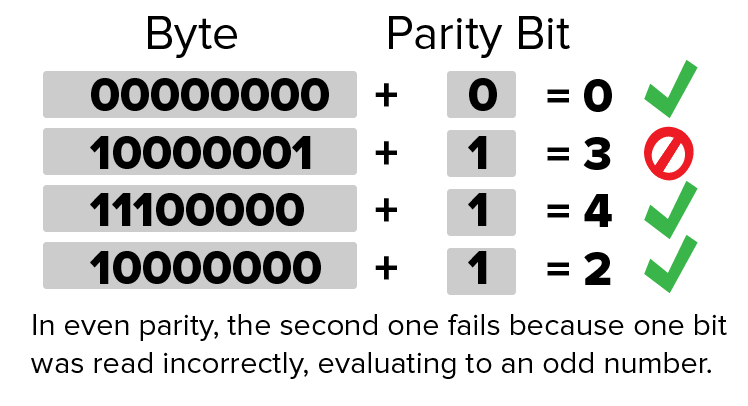
\includegraphics[width=0.9\linewidth]{Grafiken/panity_transparent.png}
%			\caption{Parit�tsbit}
%		\end{figure}
%	\end{frame}


%	\subsection{Grundlagen}
% 	\begin{frame}{Grundlagen}
% 	\begin{itemize}
% 		\item Was sind Wertpapiere?
% 		\begin{figure}[h]
% 				 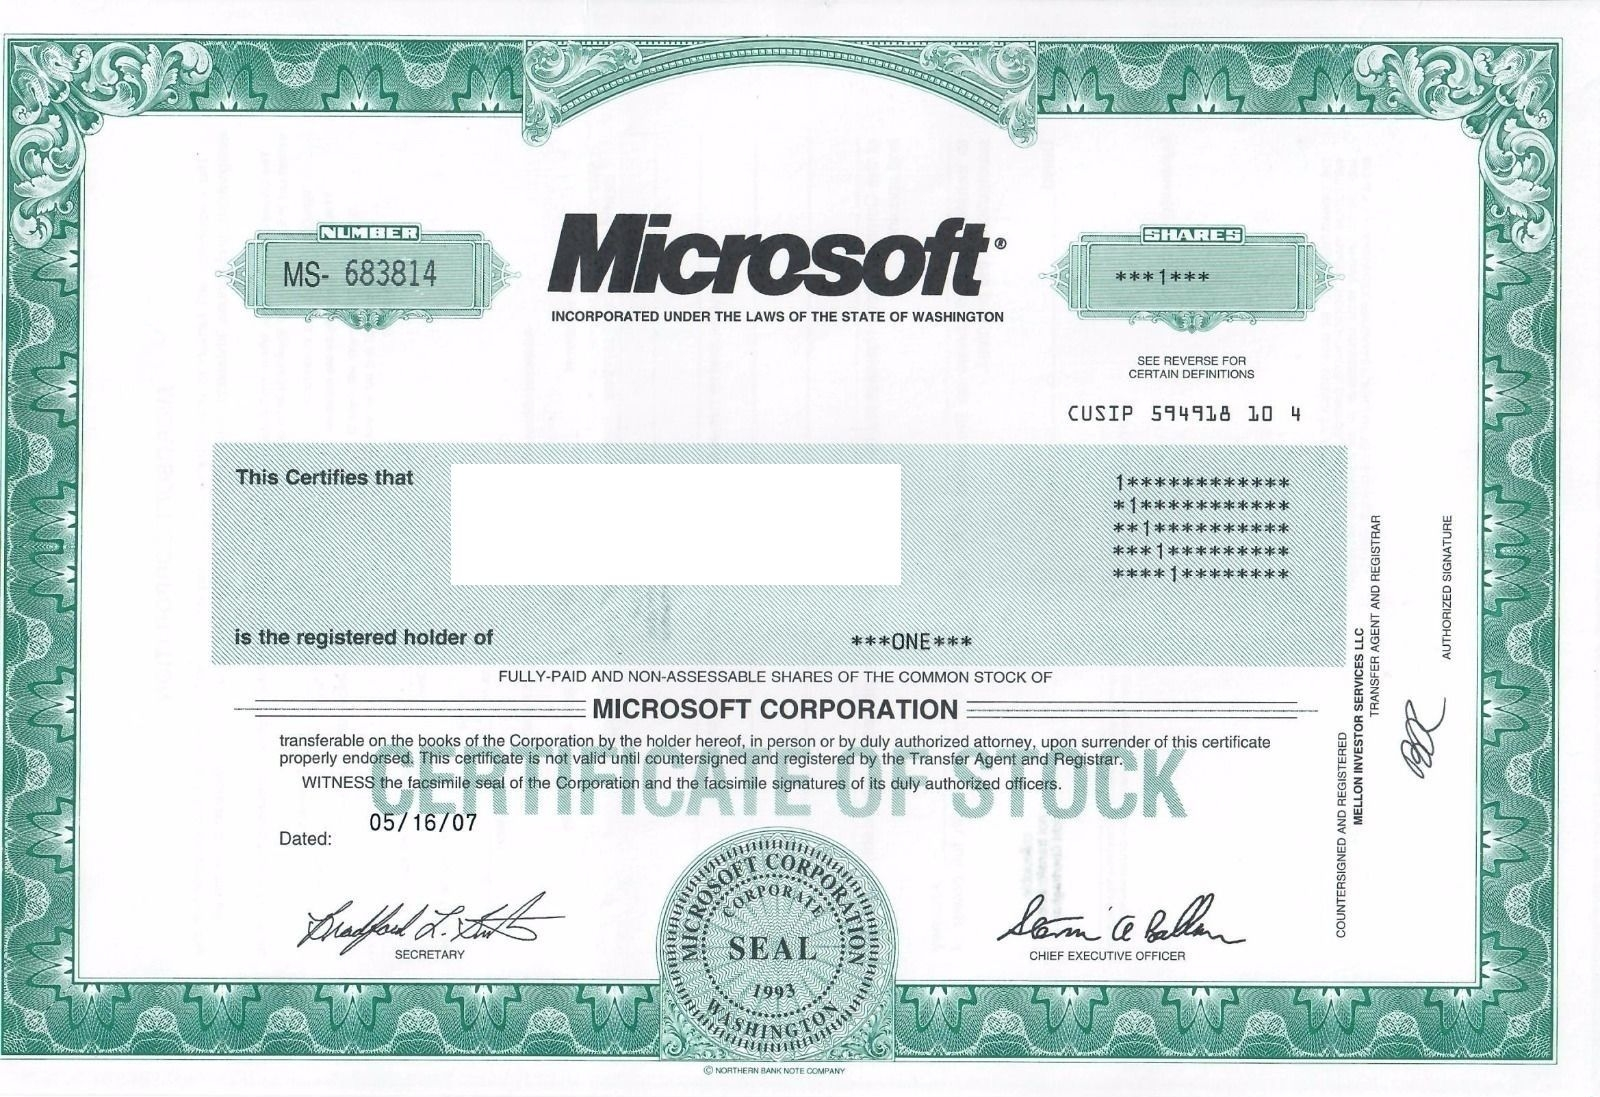
\includegraphics[width=0.45\linewidth]{Grafiken/ms-wertpapier.jpg}
% 				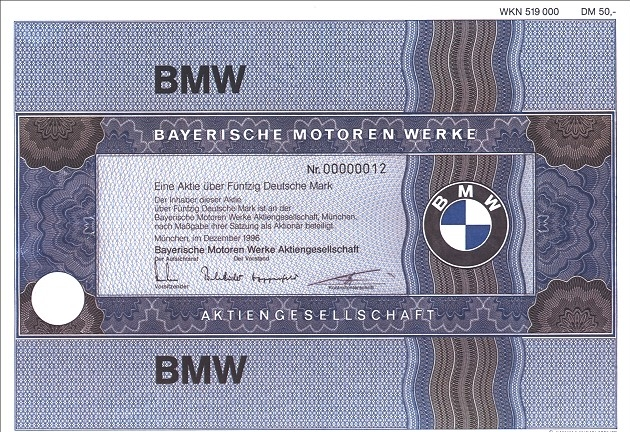
\includegraphics[width=0.45\linewidth]{Grafiken/bmw-wertpapier.jpg}
% 				\caption{Beispiele f�r Wertpapiere}
% 		\end{figure}
% 	\end{itemize}
% 	\end{frame}
 
 
%	\subsection{Code}
%	\begin{frame}[fragile]{Code}
%		\begin{lstlisting}
%def ISIN_2_quersum(ISIN_in):
%
%for i in range(0, len(ISIN_in)):
%  quersumme = ""
%  quersumme_out = 0
%  if len(ISIN_in)%2 == 1:
%	if i%2 == 0:
%	  quersumme = quersumme + str(int(ISIN_in[i])*2)
%	else:
%	  quersumme = quersumme + ISIN_in[i]
%  else:
%    if i%2 == 1:
%        quersumme = quersumme + str(int(ISIN_in[i])*2)
%    else:
%        quersumme = quersumme + ISIN_in[i]	
%
%\end{lstlisting}
%	\end{frame}

	\section{Fazit}
		\begin{frame}{Fazit}


		\end{frame}
		
	% Endfolie
	\begin{frame}
		\vfill
		\centering
		\begin{beamercolorbox}[sep=8pt,center,shadow=true,rounded=true]{title}
			\usebeamerfont{title}Danke f�r die Aufmerksamkeit
		\end{beamercolorbox}
		\vfill
	\end{frame}
	\begin{frame}
		Quelle:\\

	\end{frame}
\end{document}